\section{Model Equations}   
The final model equations are presented in this section. \autoref{fig:boat3DForces} and \ref{fig:boat2D} show a diagram of the vessel.

\begin{figure}[H]
    \captionbox  %<--use captionbox instead if no global caption is needed
    {               %                                \%-%-%-%-%-%-%\
        Diagram of the boat where the forces applied by the motors are shown.                %\
        \label{fig:boat3DForces}                                  %\
    }                                                                 %\
    {                                                                  %\
        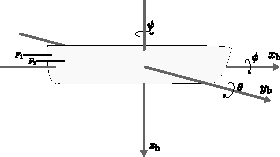
\includegraphics[width=.46\textwidth]{figures/boat3DForces}         %\
    }                                                                    %\
    \hspace{5pt}                                                          %\
    \captionbox  %<-----------------------------------------------------%\
    {       
        Above perspective of the vessel, where the distances needed for the model equations are presented.                                                                %\                         %\
        \label{fig:boat2D}                                     %\
    }                                                                           %\
    {                                                                            %\
        \includegraphics[width=.2\textwidth]{boat2D}            %|
    }                                                                             %|
\end{figure}
%
The translational movement of the vessel is describe by \autoref{eq:x_pos_model}, \ref{eq:y_pos_model} and \ref{eq:z_pos_model}.
%
\begin{flalign}
    m \ddot{x}_\mathrm{b} &=  F_\mathrm{1} + F_\mathrm{2}  - d_{\dot{x}_\mathrm{b}} \dot{x}_\mathrm{b} + F_{x_\mathrm{b}}
    \label{eq:x_pos_model} \\
    m \ddot{y}_\mathrm{b} &=  -d_{\dot{y}_\mathrm{b}} \dot{y_\mathrm{b}} + F_{y_\mathrm{b}}
    \label{eq:y_pos_model} \\
    m \ddot{z}_\mathrm{b} &=  -d_{\dot{z}_\mathrm{b}}\dot{z_\mathrm{b}} + F_{z_\mathrm{b}} \label{eq:z_pos_model}
\end{flalign}
%
\begin{where}
    \va{m}{is the mass of the vessel}{kg}
%    \va{m_\mathrm{x}}{}{kg}
%    \va{m_\mathrm{y}}{}{kg}
%    \va{m_\mathrm{z}}{}{kg}
    \va{\ddot{x}_\mathrm{b}}{is the acceleration in the $x_\mathrm{b}$ direction}{m s^{-2}}
    \va{\ddot{y}_\mathrm{b}}{is the acceleration in the $y_\mathrm{b}$ direction}{m s^{-2}}
    \va{\ddot{z}_\mathrm{b}}{is the acceleration in the $z_\mathrm{b}$ direction}{m s^{-2}}
    \va{\dot{x}_\mathrm{b}}{is the velocity in the $x_\mathrm{b}$ direction}{m s^{-1}}
    \va{\dot{y}_\mathrm{b}}{is the velocity in the $y_\mathrm{b}$ direction}{m s^{-1}}
    \va{\dot{z}_\mathrm{b}}{is the velocity in the $z_\mathrm{b}$ direction}{m s^{-1}}
    \va{F_1}{is the force applied by motor 1}{N}
    \va{F_2}{is the force applied by motor 2}{N}
\end{where}
    
The translational movement of the vessel is describe by \autoref{eq:phi_model}, \ref{eq:theta_model} and \ref{eq:psi_model}.

\begin{flalign}
    I_\mathrm{x}\ddot{\phi} &= -d_{\dot{\phi}} \dot{\phi} + T_\mathrm{\phi}  
    \label{eq:phi_model} \\
    I_\mathrm{y}\ddot{\theta} &= -d_{\dot{\theta}} \dot{\theta} + T_\mathrm{\theta}  
    \label{eq:theta_model} \\
    I_\mathrm{z}\ddot{\psi} &= F_\mathrm{1}l_\mathrm{1} - F_\mathrm{2} l_\mathrm{2} - d_{\dot{\psi}} \dot{\psi} + T_\mathrm{\psi} \label{eq:psi_model}
\end{flalign}
%
\begin{where}
    \va{I_\mathrm{x}}{is the inertia around the $x_\mathrm{b}$ axis}{kg}
    \va{I_\mathrm{y}}{is the inertia around the $y_\mathrm{b}$ axis}{kg}
    \va{I_\mathrm{z}}{is the inertia around the $z_\mathrm{b}$ axis}{kg}
    \va{\ddot{\phi}}{is the angular acceleration around the $x_\mathrm{b}$ axis}{rad s^{-2}}
    \va{\ddot{\theta}}{is the angular acceleration around the $y_\mathrm{b}$ axis}{rad s^{-2}}
    \va{\ddot{\psi}}{is the angular acceleration around the $z_\mathrm{b}$ axis}{rad s^{-2}}
    \va{\dot{\phi}}{is the angular velocity around the $x_\mathrm{b}$ axis}{rad s^{-1}}
    \va{\dot{\theta}}{is the angular velocity around the $y_\mathrm{b}$ axis}{rad s^{-1}}
    \va{\dot{\psi}}{is the angular velocity around the $z_\mathrm{b}$ axis}{rad s^{-1}}
    \va{l_1}{is the perpendicular distance from motor 1 to the center of gravity}{m}
    \va{l_2}{is the perpendicular distance from motor 2 to the center of gravity}{m}
\end{where}


%\begin{flalign}
%    m_\mathrm{x} \ddot{x}_\mathrm{b} &=  F_\mathrm{1} + F_\mathrm{2}  - d_\mathrm{x} \dot{x}_\mathrm{b} + m_\mathrm{y} \dot{y_\mathrm{b}} \dot{\psi} - m_\mathrm{z} \dot{z}_\mathrm{b} \dot{\theta} - F_\mathrm{x}
%    \label{eq:x_pos_model} \\
%    m_\mathrm{y} \ddot{y_\mathrm{b}} &=  -d_\mathrm{y}\dot{y_\mathrm{b}}-m_\mathrm{x}\dot{x_\mathrm{b}}\dot{\psi}+m_\mathrm{z}\dot{z_\mathrm{b}}\dot{\phi}-F_\mathrm{y}
%    \label{eq:y_pos_model} \\
%    m_\mathrm{z} \ddot{z_\mathrm{b}} &=  -d_\mathrm{z}\dot{z_\mathrm{b}}+ m_\mathrm{b}\dot{x_\mathrm{b}}\dot{\theta}-m_\mathrm{y}\dot{y_\mathrm{b}} \dot{\phi}-F_\mathrm{z} \label{eq:z_pos_model}
%\end{flalign}
%
%\begin{flalign}
%    I_\mathrm{x}\ddot{\phi} &= -d_\mathrm{\phi} \dot{\phi}-(m_\mathrm{z}-m_\mathrm{y}) \dot{z}_\mathrm{b} \dot{y}_\mathrm{b}-(I_\mathrm{z}-I_\mathrm{y}) \dot{\theta } \dot{\psi}+T_\mathrm{\phi}  
%    \label{eq:x_inert_model} \\
%    I_\mathrm{y}\ddot{\theta} &= -d_\mathrm{\theta} \dot{\theta}-(m_\mathrm{z}-m_\mathrm{x}) \dot{x}_\mathrm{b} \dot{y}_\mathrm{b}-(I_\mathrm{x}-I_\mathrm{z}) \dot{\phi} \dot{\psi}+T_\mathrm{\theta}  
%    \label{eq:y_inert_model} \\
%    I_\mathrm{z}\ddot{\psi} &= -d_\mathrm{\psi} \dot{\psi}-(m_\mathrm{y}-m_\mathrm{x}) \dot{x}_\mathrm{b}\dot{y}_\mathrm{b}-(I_\mathrm{z}-I_\mathrm{y})\dot{\psi}\dot{\theta}+F_\mathrm{1}l_\mathrm{1}+F_\mathrm{2}l_\mathrm{2}+T_\mathrm{\psi} \label{eq:z_inert_model}
%\end{flalign}
